\documentclass[final,5p,times,twocolumn]{elsarticle}
\usepackage[T1]{fontenc}
\usepackage{amsmath,amssymb,amsthm,booktabs,tabularx,longtable,array,graphicx}
\usepackage{enumitem,xcolor,tikz,microtype,xurl,algorithm,algpseudocode,fancyhdr}
\usepackage[hidelinks]{hyperref}
\usetikzlibrary{arrows.meta,positioning,fit,backgrounds,calc}
\definecolor{ink}{HTML}{183A45}
\definecolor{teal}{HTML}{087F7A}
\definecolor{blue}{HTML}{405F8A}
\newcolumntype{P}[1]{>{\raggedright\arraybackslash}p{#1}}
\newcolumntype{Y}{>{\raggedright\arraybackslash}X}
\newtheorem{proposition}{Proposition}[section]
\newtheorem{theorem}[proposition]{Theorem}
\newtheorem{corollary}[proposition]{Corollary}
\newtheorem{lemma}[proposition]{Lemma}
\newcommand{\E}{\mathbb E}
\newcommand{\TV}{\operatorname{TV}}
\newcommand{\Var}{\operatorname{Var}}
\newcommand{\Cov}{\operatorname{Cov}}
\newcommand{\BQ}{GeoI-BQ}
\setlength{\emergencystretch}{2em}
\setlength{\tabcolsep}{3.5pt}
\renewcommand{\arraystretch}{1.06}
\setlength{\textfloatsep}{10pt plus 2pt minus 2pt}
\setlength{\dbltextfloatsep}{10pt plus 2pt minus 2pt}
\setlength{\floatsep}{8pt plus 2pt minus 2pt}
\setlength{\dblfloatsep}{8pt plus 2pt minus 2pt}
\setlist{nosep,leftmargin=*}
\renewcommand{\topfraction}{.95}
\renewcommand{\textfraction}{.04}
\renewcommand{\floatpagefraction}{.8}
\setcounter{topnumber}{5}
\setcounter{dbltopnumber}{5}
\renewcommand{\dbltopfraction}{.95}
\setcounter{totalnumber}{5}
\raggedbottom
\fancypagestyle{pprintTitle}{\fancyhf{}\fancyfoot[C]{\thepage}\renewcommand{\headrulewidth}{0pt}}
\hypersetup{pdftitle={GeoI-BQ: Bounded Transcript Disclosure for Road-Aware Location Queries},
pdfauthor={Hanh Ngo-Minh; Phan Trong Nhan},pdfsubject={Research manuscript; affiliations and contact details pending}}
\begin{document}
\begin{frontmatter}
\title{GeoI-BQ: Bounded Transcript Disclosure for Road-Aware Location Queries}
\author{Hanh Ngo-Minh}
\author{Phan Trong Nhan}
\begin{abstract}
Repeated location queries expose a transcript whose privacy cannot be inferred from
isolated noisy points. We present GeoI-BQ, combining a geo-indistinguishable road
reference, private reference reuse and bounded joint query-segment sampling.
A summable allowance schedule limits transcript disclosure without specifying trip
duration. Under explicit support, timing, state and provider assumptions, we derive
an end-to-end likelihood-ratio bound and prior-dependent localization guarantees.
Utility analysis separates planning-score gain from actual service reward and bounds
deviation from a matched public base. A controlled synthetic comparison with three
audited paper adaptations and two controls uses 20 test families and 120 retained
trip-draws. GeoI-BQ achieves 99.595\% session Recall@5 and 0--0.188\% Hit100 across
five localization tasks, using 155 coordinate queries per 600-second session.
The nonadaptive base has slightly higher Recall, and complete static-reference
access limits claims of online necessity. These findings support a conditional
transcript mechanism and reproducible trade-off analysis, rather than deployment
certification or faithful reproduction of the original papers.

\end{abstract}
\begin{keyword}
Trajectory privacy \sep Geo-indistinguishability \sep Location-based services \sep
Adaptive composition \sep Point-of-interest retrieval
\end{keyword}
\end{frontmatter}
\hypersetup{pdfauthor={Hanh Ngo-Minh; Phan Trong Nhan}}
\section{Introduction}\label{sec:intro}
Location-based services (LBSs) connect private movement to remote information retrieval. A
device may request nearby facilities repeatedly, and a provider can combine the resulting
coordinates, timestamps and replies with road geometry and prior knowledge. Correlation across
requests matters: a plausible replacement at one instant may become identifiable when the
complete sequence is examined. The uniqueness of mobility traces motivates this concern,
although observations on real populations do not automatically transfer to synthetic
trajectories or to physical identities~\cite{mobilityunique}.

Geo-indistinguishability (Geo-I) expresses location privacy through a likelihood-ratio bound
scaled by input distance~\cite{geoi}. Extending that guarantee to an implemented continuous
service requires accounting for more than repeated noise generation. Decisions to reuse a
reference, the construction of query candidates, the sampling of public actions, retries and
session boundaries can each depend on private information. Predictive private mechanisms
already show the importance of managing new information over time~\cite{predictive}.
Our focus is the explicit connection between these mechanisms and the transcript actually
observed by an LBS provider.

Utility also requires a task definition. A coordinate close to a user may retrieve poor
answers across a one-way road or a travel-time boundary. Conversely, several remote query
locations can recover useful metadata that the device ranks accurately using its current
GPS. Prior work combines Geo-I, dummy queries and local processing in application-specific
settings~\cite{ev}. Thus neither multiple queries nor local selection alone is our novelty
claim. The question is how to specify a stateful publication policy, bound its complete
transcript, and evaluate its answers without confusing a planning proxy with service utility.

Comparability is another obstacle. Recent methods release a replacement coordinate, a set
containing the true location and dummies, or extra fake packets; offline trajectory generation
has a different output contract~\cite{transprotect,semantic,fake,sok}. A real-member anonymity
metric does not apply unchanged to a query set that need not contain the true location.
We therefore retain task-aligned localization and service metrics alongside original metrics
where their definitions and required inputs remain applicable. We do not propose new formulas
for mean absolute error (MAE), Recall or bootstrap intervals.

We examine \BQ{}, a family of policies with Geo-I cap $C_s$ and query allowance $\Gamma_Q$;
the evaluated v1 configuration remains fixed throughout this article. A road exponential
mechanism and a private reuse test maintain an internal reference $Z$. An approximate belief
computed from protected history scores a common library of road-feasible query segments.
A bounded centered kernel selects one segment; its frames are then released at public times.
The device retrieves a purpose-independent cover, caches valid metadata, and returns a full
filtered and sorted local answer.

The information-access model is consequential. The present prototype loads a complete
public reference that matches the static provider used in the experiment. Its utility
evaluation restricts answers to received candidates, but does not establish that an
operational device lacks the information to answer offline. Likewise, a nonadaptive public
base has slightly higher Recall in this cohort. We preserve these adverse findings.
They limit claims about application necessity and the benefit of private adaptation, while
leaving the conditional transcript analysis meaningful.

The article makes three scoped contributions:
\begin{enumerate}[leftmargin=*,itemsep=3pt]
\item A road-aware, stateful publication policy with separate accounting for private GPS
operations and bounded joint query-segment selection. The analysis covers the ordered
transcript under stated support, clock, provider and state assumptions.
\item A connected privacy--utility analysis: an end-to-end likelihood-ratio bound, a
prior-concentration corollary for arbitrary-estimator localization, conditional composition
of multiple channels, and utility statements that separate exact properties from
uncertified calibration assumptions.
\item A reproducible controlled comparison with three audited paper adaptations and two
controls, accompanied by supplementary inference tasks, family-level uncertainty, cost
accounting and an audit of catalogue saturation and the untested cap-exhausted regime.
\end{enumerate}
We do not claim to be the first road-aware Geo-I mechanism, to outperform every original
paper implementation, or to certify a complete deployed system.
Section~\ref{sec:related} positions the work; Section~\ref{sec:method} specifies and analyzes
the method; Section~\ref{sec:evaluation} reports the comparison and its limits; and
Section~\ref{sec:conclusion} concludes.

\section{Related work}\label{sec:related}
\subsection{Spatial guarantees and protected mobility history}
Geo-I bounds the relative probability of an output under two candidate locations, using a
spatial metric~\cite{geoi}. Predictive mechanisms extend the discussion to mobility traces
by distinguishing predicted behavior from information that requires a new private
measurement~\cite{predictive}. Composition and post-processing provide the general
mathematical tools~\cite{dworkroth}; they do not justify unaccounted private candidate pruning
or a GPS-dependent send decision.

Road constraints and utility-aware querying are established directions. The electric-vehicle
querying mechanism of Atmaca et al.\ combines approximate Geo-I with dummy requests and
local processing~\cite{ev}. Road-aware personalized protection under spatiotemporal
correlation is also studied in PTPPM~\cite{ptppm}. These precedents rule out treating
road awareness, mobility prediction or local selection by themselves as distinctive
contributions. Our analysis concerns the particular common-support segment kernel and
its connection to complete transcript disclosure and answer-level utility.

The IWPE 2026 program also lists a road-adaptive, mobility-prediction mechanism
by Santos et al.~\cite{iwpe26}. Its abstract describes dynamic budget allocation
and grouping by predicted proximity. We use this program abstract to delimit
overlap, without inferring an unavailable full specification or a reproducible
comparator. The distinctive claim here is the specified bounded publication
channel and its connected analysis, rather than combining prediction with roads.

\subsection{Replacement coordinates, dummy sets and inserted queries}
TransProtect uses contextual prediction and utility information to construct synthetic
vehicle locations~\cite{transprotect}. Its replacement-coordinate contract supports
coordinate inference error and travel-cost distortion measurements. Our comparison uses
a Markov adaptation in place of its neural predictor; results must therefore be read
as implementation-specific controlled evidence.

Semantic-correlation dummy schemes generate sets containing the true point and plausible
alternatives~\cite{semantic}. Temporal and semantic consistency can make dummy paths
less easily discarded, but true-member inference remains a distinct task. The semantic
source and empirical predictor in our adaptation differ from the paper's original setting.
Fake-query insertion adds dummy-only events between genuine requests~\cite{fake}.
Its benefits depend partly on the observer's knowledge of timing. We preserve natural
extra events, allow the attacker to know the public service clock, and count every
emitted query. This is a declared threat-model choice, not a reproduction of the
original paper's anonymity scores.

\subsection{Identity, correlated channels and offline publication}
Pseudonym and beacon protection in vehicular networks, such as CPCROK~\cite{cpcrok},
addresses linkability under communication contracts different from online POI retrieval.
A query mechanism does not automatically remove an account, network identifier or
physical vehicle identity. Our route-family association task is explicitly a proxy.
DP-FETC studies differentially private trajectory publication using features and
correlations~\cite{dpfetc}; distributional fidelity of an offline release is not the
same quantity as online localization error. The SoK by Buchholz et al.\ emphasizes
the difficulty of reconciling trajectory privacy, utility and evaluation
assumptions~\cite{sok}.

\begin{table}[htbp]\centering\footnotesize
\caption{Recent related work: contracts, task coverage and evidence status.}\label{tab:related}
\begin{tabularx}{\linewidth}{@{}P{2.5cm}P{2.05cm}P{2.15cm}YP{2.35cm}@{}}\toprule
\textbf{Work} & \textbf{Output} & \textbf{Coverage} & \textbf{Privacy / utility metrics} & \textbf{This study} \\
\midrule
TransProtect (2024)\cite{transprotect} & Synthetic coordinate & D: S1, S3; P: S2 & EIE / VehiTrack; travel-cost distortion & Markov adaptation \\
Semantic (2026)\cite{semantic} & Real + dummy set & D: S1; P: S2, S3 & ASR; DER; generation time & OSM/empirical adaptation \\
Fake queries (2026)\cite{fake} & Mixed and fake-only sets & D: S1, S3; P: S2 & ASR; indistinguishable paths; runtime/RSS & Road/history adaptation \\
EV querying (2024)\cite{ev} & Noisy/dummy queries & P: S1--S3 & Approx.\ Geo-I; IBU/Wasserstein; cost of privacy & Survey only; Edge contract differs \\
CPCROK (2025)\cite{cpcrok} & Pseudonyms / beacons & P: S4 & Relinking; fake routes; communication & Different VANET contract \\
DP-FETC (2025)\cite{dpfetc} & Offline trajectory data & P: S3, S8--S10 & DP; mutual information; JSD & Different release contract \\
PTPPM (2025)\cite{ptppm} & Road perturbation & U: S1, S3 & Geo-I; distortion / QoS & Preprint; no audited comparator \\
SoK (2024)\cite{sok} & Synthesis survey & Not a comparator & Privacy units; reconstruction; utility & Context and evaluation guidance \\
\bottomrule\end{tabularx}
\par\smallskip\raggedright D: directly evaluated task under source assumptions; P: partial overlap; U: insufficient audited evidence for a stronger mapping. Unlisted scenarios have no direct coverage established here. D does not imply universal protection.
\end{table}

Table~\ref{tab:related} summarizes the relevant contracts. The recent-method survey retains
its audited publication window, 28 October 2023--28 October 2026; older works supply
foundations. It is a targeted comparison, not an exhaustive systematic review.
The gap addressed here is a connected specification and analysis of a bounded segment
policy, together with an inspectable evaluation across compatible tasks. Original
metrics remain valuable; unavailable posterior models, similarity rules or output
contracts are not silently replaced by renamed localization scores.

\section{Proposed method and analysis}\label{sec:method}
\subsection{System, private inputs and information access}\label{sec:system}
Let $V$ be a finite directed road-state space with coordinates $a_v$ in a fixed metric
projection. Distinct lane states may have identical coordinates. We use Euclidean distance
for Geo-I and localization error; directed road cost is a separate quantity used for
feasibility and service ranking. A trajectory $X=(x_0,x_1,\ldots)$ is defined at all
potential protected-read times on a common clock, including times skipped by the filter.
For two trajectories,
\begin{equation}
D_\infty(X,X')=\sup_i\|x_i-x_i'\|_2. \label{eq:metric}
\end{equation}
This is the deviation between synchronized hypotheses, not distance traveled.

The true request $\psi_t$ contains purpose, category and local parameters, such as a radius
or destination. GPS and $\psi_t$ remain local. The provider sees the ordered transcript
$O_n$ of coordinates, timestamps, common requests, responses and retries after $n$ segment
selections. It does not receive $Z$, belief, private ledger, refresh flags or ranked local
answers. We consider a provider that knows the algorithm and public context $C$.
Account/IP identifiers, application feedback and private start/stop timing require
additional channels and are not silently covered.

Figure~\ref{fig:system} locates the mechanism in the system. Information access must be
distinguished from publicity: a public catalogue is not necessarily already downloaded,
but a device that possesses its complete current metadata may not need online retrieval.
In our prototype, offline reference and reply contexts are loaded into the operational
factory, and the trial provider matches that static context. The candidate mask records
what was received and permitted in the measured answer; it is not a confidentiality
barrier between an evaluator's catalogue and the client.

\begin{figure}[htbp]\centering
\resizebox{\linewidth}{!}{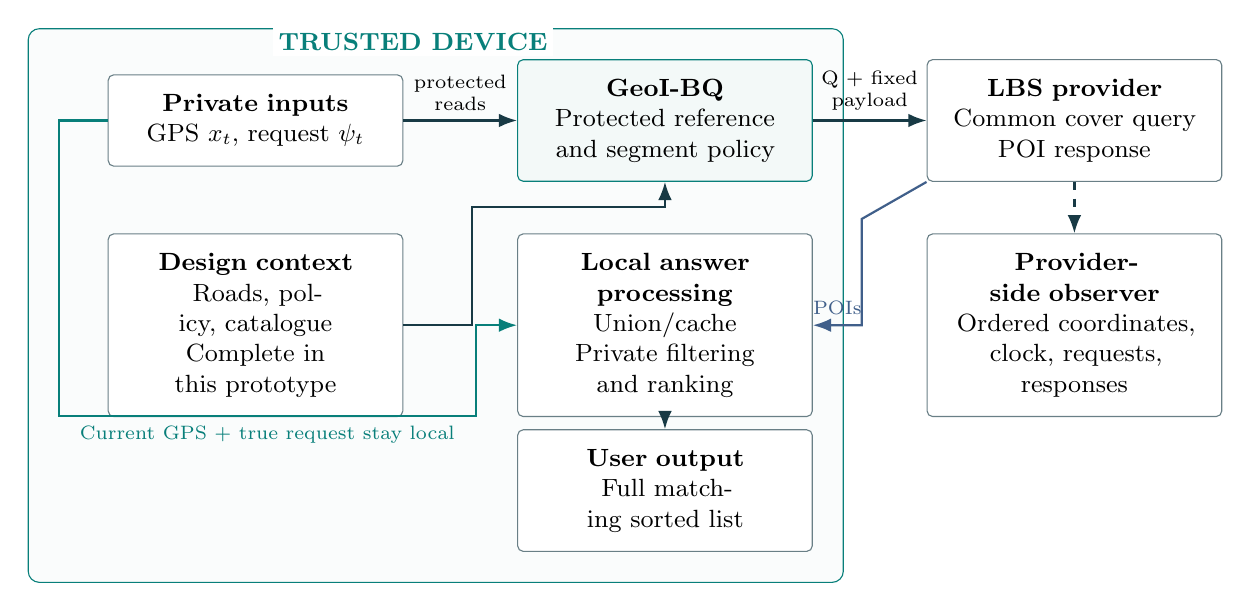
\begin{tikzpicture}[>=Latex,
 box/.style={draw=ink!65,rounded corners=2pt,fill=white,text width=3.25cm,
 align=center,inner sep=7pt,font=\small},
 arr/.style={->,thick,draw=ink}]
\node[box] (input) at (0,0) {\textbf{Private inputs}\\GPS $x_t$, request $\psi_t$};
\node[box,draw=teal,fill=teal!5] (model) at (5.2,0)
{\textbf{GeoI-BQ}\\Protected reference\\and segment policy};
\node[box] (server) at (10.4,0)
{\textbf{LBS provider}\\Common cover query\\POI response};
\node[box] (context) at (0,-2.6)
{\textbf{Design context}\\Roads, policy, catalogue\\Complete in this prototype};
\node[box] (local) at (5.2,-2.6)
{\textbf{Local answer processing}\\Union/cache\\Private filtering and ranking};
\node[box] (attacker) at (10.4,-2.6)
{\textbf{Provider-side observer}\\Ordered coordinates,\\clock, requests, responses};
\node[box] (output) at (5.2,-4.7)
{\textbf{User output}\\Full matching sorted list};
\draw[arr] (input)--node[above,font=\scriptsize,text width=1.35cm,align=center]{protected\\reads}(model);
\draw[arr] (model)--node[above,font=\scriptsize,text width=1.35cm,align=center]{Q + fixed\\payload}(server);
\draw[arr] (context.east)--(2.75,-2.6)--(2.75,-1.1)--(5.2,-1.1)--(model.south);
\draw[arr,blue] (server.south west)--(7.7,-1.25)--(7.7,-2.6)--
node[above,font=\scriptsize]{POIs}(local.east);
\draw[arr] (local)--(output);
\draw[arr,dashed] (server)--(attacker);
\draw[arr,teal] (input.west)--(-2.5,0)--(-2.5,-3.75)--
node[below,font=\scriptsize]{Current GPS + true request stay local}(2.8,-3.75)
--(2.8,-2.6)--(local.west);
\coordinate (corner) at (-2.5,-3.75);
\begin{scope}[on background layer]
\node[fit=(input)(context)(model)(local)(output)(corner),draw=teal,
 fill=teal!2,rounded corners,inner sep=11pt] {};
\end{scope}
\node[font=\small\bfseries,text=teal,fill=white,inner sep=2pt] at (2,1)
{TRUSTED DEVICE};
\end{tikzpicture}
}
\caption{System boundary and information flow. The complete design context is available in
the present prototype. An operational proxy--provider separation would require explicit
unknown metadata and a matching service evaluation.}\label{fig:system}
\end{figure}

Accordingly, the experiment measures received-candidate quality under a declared acquisition
contract. If the same complete valid POI records and road costs are already usable locally,
all four evaluated purposes can be answered offline with Recall one for every defined
reference. This analytical control does not assume free data acquisition, storage or
refresh. A production setting with a public proxy $\widehat{\mathcal D}$ and unknown
current provider records $\mathcal D_t$ is a different information contract; dynamic
attributes cannot retrospectively justify the static trial.

\subsection{Assumptions for transcript guarantees}\label{sec:assumptions}
We make the following requirements explicit.
\begin{enumerate}[label=A\arabic*.,leftmargin=*,itemsep=3pt]
\item At the same public context and augmented action history, the candidate segment
library, ordering and positive base masses are identical. GPS, $Z$, belief and private
request do not prune support. Within the valid public domain, a common stationary
segment supplies holding feasibility.
\item The spatial guarantee uses ideal REM and private-test kernels; downstream reads
only their protected history and permitted context. All new private reads are accounted
before access. Restarts must restore the full required upstream state, not merely a clock.
\item The query kernel receives scores in $[0,1]$ and samples its integer PMF using fresh
uniform bits. Its random source is independent of private input and upstream randomness.
\item Actions and allowance counters are committed before publication and cannot roll
back within a session. Clock and session boundaries are common when inputs are compared,
or follow a public-history-only rule. Subsequent frames and retries reuse the action.
\item At the same public query/history, the provider has the same conditional response
law under either private input. Private GPS or intent creates no additional request.
\item Cache/ranking results require valid, sufficient metadata and the same local
request and total order. Transfer to actual service utility requires separately justified
proxy and distribution error bounds.
\end{enumerate}
Augmented history includes selected fake lane states as well as public coordinates:
coordinate aliases need not identify subsequent feasible transitions. We prove a bound
on this stronger history before projecting to the wire. Movement and future targets
are fixed exogenously for the analysis; user decisions altered by service replies
would require an interactive feedback model.

\subsection{Protected references and prospective accounting}
With a common road domain, the road exponential mechanism (REM) samples
\begin{equation}
R_u(v\mid x)=
\frac{\exp[-u\|x-a_v\|_2/2]}{\sum_{w\in V}\exp[-u\|x-a_w\|_2/2]},
\qquad Z=a_v,\quad v\sim R_u(\cdot\mid x). \label{eq:rem}
\end{equation}
It directly samples a road state. It is not planar noise followed by a second matching
step. A GPS-dependent truncation of $V$ would require a different proof.
After the first reference, a permitted read tests an old reference $h$:
\begin{equation}
D_t=\mathbf1\{\|x_t-h\|_2+\xi_t>\theta\},\qquad
\xi_t\sim\operatorname{Lap}(0,1/u). \label{eq:test}
\end{equation}
A zero result reuses $h$; otherwise REM refreshes it. The initial release costs one
unit $u$, test-and-reuse one unit, and test-and-refresh two units.

For a session cap $C_s>0$, choose $0<u\le C_s$ and $M=\lfloor C_s/u\rfloor$.
The prospective filter preserves
\begin{equation}
\operatorname{Spent}_n=u\sum_{i=0}^n c_i\le Mu\le C_s,\qquad c_i\in\{0,1,2\}. \label{eq:cap}
\end{equation}
It reserves the maximal possible next cost before reading GPS. A skipped read cannot
itself be selected by an unaccounted GPS test. The frozen configuration parameterizes
$u=B/(2H_{\rm cfg})$, $M=2H_{\rm cfg}-1$ with $B=0.24\,\mathrm m^{-1}$ and
$H_{\rm cfg}=12$, giving $u=0.01\,\mathrm m^{-1}$ and effective cap
$C_s=0.23\,\mathrm m^{-1}$. These are configuration values, not a universal risk policy.
Exhaustion prevents further protected GPS input; it does not force query termination.
More generally, a sufficient spatial policy for likelihood ratio at most $R_\star>1$
throughout a declared neighborhood $D_\infty\le d_\star$ is
$C_s\le\log(R_\star)/d_\star$. This converts a stated distinguishability target
into a cap; it does not justify the frozen numerical cap without such a policy
or promise a fixed number of useful future observations.

\subsection{Protected belief and common segment library}
An approximate belief over representative states predicts and updates as
\begin{align}
b_t^-(s)&=\sum_r b_{t-1}(r)T_{\Delta t}(r,s),\\
b_t(s)&=\frac{b_t^-(s)\ell_t(Z_t\mid s,h)}
                    {\sum_r b_t^-(r)\ell_t(Z_t\mid r,h)}. \label{eq:belief}
\end{align}
At an update, the emission combines the reuse atom and refresh:
$\ell(z\mid s,h)=r_s\mathbf1_{\{z=h\}}+
(1-r_s)\sum_{v:a_v=z}R_u(v\mid s)$, where $r_s$ is the reuse probability.
Without a private read, prediction alone is performed; a repeated reference is not
treated as an independent new REM observation. State discretization, prior and motion
transitions are public approximations, not a certified posterior of a real user.

An action $A_a$ is a segment with three frames, each containing $K=5$ fake road states.
Frame transitions respect directed-road feasibility from previously selected fake
states. Public search and cover goals generate a common library
$\mathcal A_j(\mathcal H_{j-1})$. Belief changes scores, not the library or positive
base masses $w_a$. Holding is a feasible common action in the declared domain.
The frozen initial policy filters only by a public reference-mass floor;
an empty public goal/filter domain raises a reported construction failure,
rather than relaxing support using private information. The trial has no such failure.
The evaluated planner uses a portfolio width of 24, novelty and long-range weights
of four, and a 60-second travel scale. These are frozen choices, not proven optima.
The supplement specifies the cache-coverage/proximity score and public masses.

\subsection{Bounded joint sampling, publication and local answers}
From a bounded public proxy $g_a(s)$, compute raw score $v_a=\sum_s b(s)g_a(s)$.
Normalization and quantization give $z_a=F_a/S\in[0,1]$, $S=65536$.
The centered kernel is
\begin{align}
\varepsilon_{Q,j}&=\frac{\Gamma_Q}{j(j+1)},&
\alpha_j&=\frac{\widehat\varepsilon_{Q,j}}{2+\widehat\varepsilon_{Q,j}},\\
\mu_j&=\sum_a w_a z_a,&
p_a&=w_a[1+\alpha_j(z_a-\mu_j)]. \label{eq:kernel}
\end{align}
Here $0\le\widehat\varepsilon_{Q,j}\le\varepsilon_{Q,j}$ is the exact rational
value obtained by rounding the scheduled allowance downward to binary64
before constructing the integer kernel. The nominal schedule remains a valid upper bound.
The evaluated allowance is $\Gamma_Q=1$. Min--max normalization can change the score
scale; $z_a$ is neither actual Recall nor a calibrated GPS probability. The proof uses
its bounded range, not an unjustified sensitivity claim.

With $w_a=m_a/T$ and $\alpha_j=N/D$, exact finite sampling uses
\begin{equation}
W_a=m_a\left[DTS+N\left(TF_a-\sum_c m_cF_c\right)\right],
\qquad \sum_aW_a=DT^2S. \label{eq:integer}
\end{equation}
A uniform integer below the total mass selects its cumulative interval.
The representation avoids floating cumulative probabilities; it does not certify
the simulator's entropy source or the upstream floating-point mechanism.

A selected segment is committed once and emitted at offsets 0, 20 and 40 seconds.
The next segment begins at 60 seconds. The protected layer reads fresh GPS no more
often than every 60 seconds and only when its prospective filter allows it.
Current GPS can still be used privately for local ranking at service ticks.
Thus protected-read counts are not total GNSS activations or energy measurements.
Every public coordinate requests the same six categories with response depth $L=60$
per category. The true purpose, category, radius and destination remain local.
Received metadata are deduplicated by POI identifier and cached under the declared
validity rule. The application returns the full matching sorted list; top five
defines only the evaluation reference.

\begin{figure}[htbp]\centering
\resizebox{.93\linewidth}{!}{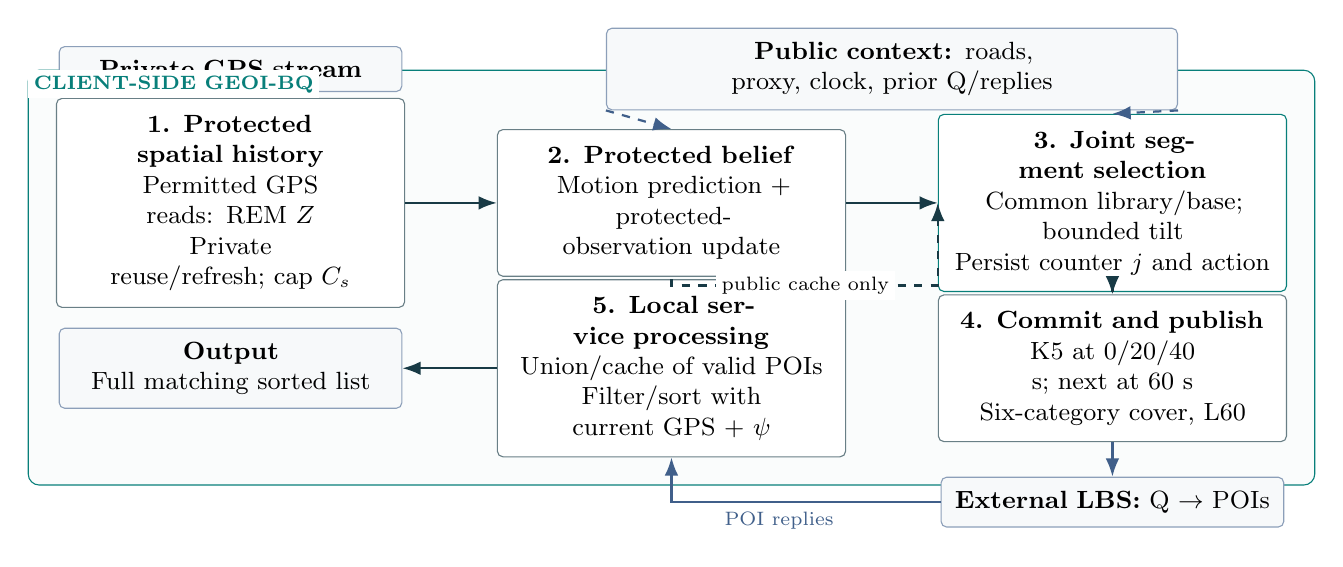
\begin{tikzpicture}[>=Latex,
 box/.style={draw=ink!65,rounded corners=2pt,fill=white,text width=4cm,
 align=center,inner sep=6pt,font=\small},
 side/.style={draw=blue!60,fill=blue!4,rounded corners=2pt,text width=4cm,
 align=center,inner sep=5pt,font=\small},
 arr/.style={->,thick,draw=ink}]
\node[box] (rem) at (0,0)
{\textbf{1. Protected spatial history}\\Permitted GPS reads: REM $Z$\\Private reuse/refresh; cap $C_s$};
\node[box] (belief) at (5.6,0)
{\textbf{2. Protected belief}\\Motion prediction +\\protected-observation update};
\node[box,draw=teal] (choose) at (11.2,0)
{\textbf{3. Joint segment selection}\\Common library/base; bounded tilt\\Persist counter $j$ and action};
\node[box] (send) at (11.2,-2.1)
{\textbf{4. Commit and publish}\\K5 at 0/20/40 s; next at 60 s\\Six-category cover, L60};
\node[box] (local) at (5.6,-2.1)
{\textbf{5. Local service processing}\\Union/cache of valid POIs\\Filter/sort with current GPS + $\psi$};
\node[side] (input) at (0,1.7)
{\textbf{Private GPS stream}};
\node[side,text width=6.9cm] (public) at (8.4,1.7)
{\textbf{Public context:} roads, proxy, clock, prior Q/replies};
\node[side] (output) at (0,-2.1)
{\textbf{Output}\\Full matching sorted list};
\node[side] (provider) at (11.2,-3.8)
{\textbf{External LBS:} Q $\to$ POIs};
\draw[arr] (input)--(rem);
\draw[arr] (rem)--(belief);
\draw[arr] (belief)--(choose);
\draw[arr] (choose)--(send);
\draw[arr] (local)--(output);
\draw[arr,blue] (send)--(provider);
\draw[arr,blue] (provider.west)-|node[below,pos=.3,font=\scriptsize]{POI replies}(local.south);
\draw[arr,dashed,blue] (public.south west)--(belief.north);
\draw[arr,dashed,blue] (public.south east)--(choose.north);
\draw[arr,dashed] (local.north)--(5.6,-1.05)-|(choose.west);
\node[font=\scriptsize,fill=white,inner sep=2pt] at (7.3,-1.05) {public cache only};
\begin{scope}[on background layer]
\node[fit=(rem)(belief)(choose)(send)(local),draw=teal,fill=teal!2,
 rounded corners,inner sep=10pt] (boundary) {};
\end{scope}
\node[font=\scriptsize\bfseries,text=teal,anchor=north west,fill=white,inner sep=2pt]
at (boundary.north west) {CLIENT-SIDE GEOI-BQ};
\end{tikzpicture}
}
\caption{GeoI-BQ workflow. One joint action produces three published frames.
Local GPS and request affect ranking, not query support or the common payload.}
\label{fig:model}
\end{figure}

\begin{algorithm}[htbp]
\caption{One public service tick of GeoI-BQ}\label{alg:policy}
\begin{algorithmic}[1]
\Require Public clock, common library policy, persisted ledgers and provider interface
\If{pacing and prospective Geo-I filter permit a protected read}
  \State Read GPS; create initial REM reference or perform private reuse/refresh
  \State Update protected history and spent units
\EndIf
\State Predict belief; apply an emission update only for an actual protected observation
\If{the tick begins a new segment}
  \State Construct the common library and positive base masses from permitted history
  \State Score using protected belief; sample by (\ref{eq:integer})
  \State Commit action, segment counter and allowance before sending
\EndIf
\State Send the committed frame with the common category cover; reuse it on retry
\State Union valid responses into cache; filter and sort locally using current GPS and $\psi_t$
\State \Return the full matching answer list
\end{algorithmic}
\end{algorithm}

For a fixed example (first trip of TEST family cache-029), the first packet
acquires 381 distinct POIs. At 20 and 40 seconds, public pacing skips a new
protected read and preserves one spent unit, even though the true GPS moves.
The first frame of the next segment at 60 seconds follows a private refresh,
raising spend to three units and cache size to 385. A further refresh at
120 seconds raises spend to five and cache size to 402; a private reuse at
180 seconds costs one additional unit and leaves the reference unchanged,
while cache size reaches 407. These internal audit labels are not provider
features. The supplement gives the retained GPS offsets, reference and Q1
coordinates; the example was selected by identifier, not by its protection score.

\subsection{Privacy of the complete transcript}\label{sec:privacy}
The following statements concern the specified ideal kernels under
Section~\ref{sec:assumptions}. They are not a certification of every floating-point
instruction in the simulator.

\begin{proposition}[REM on a common road domain]\label{prop:rem}
For any nonempty finite common $V$, (\ref{eq:rem}) is $u$-Geo-I.
Mapping the sampled road state to its coordinate preserves the bound.
\end{proposition}
\begin{proof}
Let $d=\|x-x'\|_2$, $w_x(v)=\exp[-u\|x-a_v\|_2/2]$ and
$S_x=\sum_vw_x(v)$. The reverse triangle inequality bounds
$w_x(v)/w_{x'}(v)$ by $e^{ud/2}$. Summing
$w_{x'}(v)\le e^{ud/2}w_x(v)$ over the same domain bounds $S_{x'}/S_x$
by the same factor. Their product gives $R_u(v\mid x)/R_u(v\mid x')\le e^{ud}$.
Summation proves the event bound, including coordinate aliases.
\end{proof}

\begin{proposition}[Private tests and session accounting]\label{prop:history}
Under prospective accounting, the protected history $E$ obeys
\begin{equation}
\Pr_X(E\in B)\le e^{C_sD_\infty(X,X')}\Pr_{X'}(E\in B). \label{eq:history}
\end{equation}
\end{proposition}
\begin{proof}
At a fixed protected history, $h$ is fixed and $x\mapsto\|x-h\|_2$ is
1-Lipschitz. The Laplace density ratio of the noisy distance is at most
$e^{u\|x-x'\|_2}$, so either threshold event costs one unit.
The extended reuse branch has probability $r_x$; refresh-and-state has
probability $(1-r_x)R_u(v\mid x)$. Its ratio costs at most two units.
The first reference costs one. At each common prefix the filter makes its
read decision before private access. Chain rule bounds the log ratio of any
extended history by $u\sum_i c_i\|x_i-x_i'\|_2\le C_sD_\infty$.
Marginalizing the flags and summing over the event proves (\ref{eq:history}).
No independence between successive GPS positions is assumed.
\end{proof}

\begin{proposition}[One bounded segment]\label{prop:kernel}
With common positive $w$, scores in $[0,1]$ and
$\alpha=\varepsilon/(2+\varepsilon)$, (\ref{eq:kernel}) is a positive PMF and
$p_a(b)/p_a(b')\le1+\varepsilon$ for every pair of beliefs.
\end{proposition}
\begin{proof}
Centering gives $\sum_ap_a=1$. Since $z_a-\mu\in[-1,1]$,
$w_a(1-\alpha)\le p_a\le w_a(1+\alpha)$. Dividing yields
$(1+\alpha)/(1-\alpha)=1+\varepsilon$. Conditional mixtures over random
beliefs remain in the same interval. For (\ref{eq:integer}), summing weights
cancels the centered term and yields total $DT^2S$; the normalized weight is
exactly $p_a$.
\end{proof}

\begin{proposition}[Adaptive segment composition]\label{prop:segments}
Under the common-prefix and publication assumptions, the entire ordered wire satisfies
\begin{equation}
\Pr_X(O_n\in B)\le R_n\Pr_{X'}(O_n\in B),\qquad
R_n=\prod_{j=1}^n(1+\varepsilon_{Q,j})\le e^{\Gamma_Q}. \label{eq:segments}
\end{equation}
\end{proposition}
\begin{proof}
Condition on augmented history, including fake lane states. Each action ratio is bounded
by Proposition~\ref{prop:kernel}. Provider responses have the same conditional law;
committed frames and fixed retries are post-processing. Chain rule multiplies the
action factors, and projection removes augmented state. Finally,
$\sum_{j=1}^n\varepsilon_{Q,j}=\Gamma_Q n/(n+1)$ and $1+t\le e^t$.
This argument uses conditional laws, not independent segments.
\end{proof}

The bound holds for every prefix without a known duration. For $\Gamma_Q=1$, a
rational certificate gives $R_\infty<2.437372$. Specifically,
$P_N=\prod_{j\le N}(1+1/[j(j+1)])$ and the tail sum is $1/(N+1)$.
Bounding elementary symmetric tail sums by powers of that sum yields
$R_\infty\le P_N/[1-1/(N+1)]$; $N=11$ already gives the stated outward-rounded
ceiling. The uniform cylinder-event bound also extends to an infinite transcript
under the same channel model. As $j$ grows, $\alpha_j$ vanishes and adaptation
approaches the public base; finite disclosure does not promise indefinitely
strong tracking of new GPS.

\begin{theorem}[Conditional end-to-end guarantee]\label{thm:endtoend}
If downstream uses only protected history and permitted context, and both the
spatial and Q assumptions hold, then
\begin{equation}
\Pr_X(O_n\in B)\le
\exp\!\bigl(\min\{C_sD_\infty(X,X'),\log R_n\}\bigr)
\Pr_{X'}(O_n\in B). \label{eq:endtoend}
\end{equation}
\end{theorem}
\begin{proof}
The common downstream kernel integrates the protected-history inequality
(\ref{eq:history}), giving its post-processing bound. Proposition~\ref{prop:segments}
independently bounds the same wire event. Taking the smaller ceiling proves the
claim. The two budgets are not added: $C_s$ has units $\mathrm m^{-1}$,
whereas the Q allowance is dimensionless.
\end{proof}

The Q bound can remain valid without an ideal upstream Geo-I implementation,
provided its own assumptions hold. The spatial branch requires the upstream
conditions. With the current parameters, the coarse spatial envelope crosses the
all-duration Q ceiling at $\log(2.437372)/0.23\approx3.874$ m; beyond that
distance the Q envelope is smaller. Hence strong quantitative transcript protection
must not be attributed to Geo-I alone.

\begin{figure}[htbp]\centering
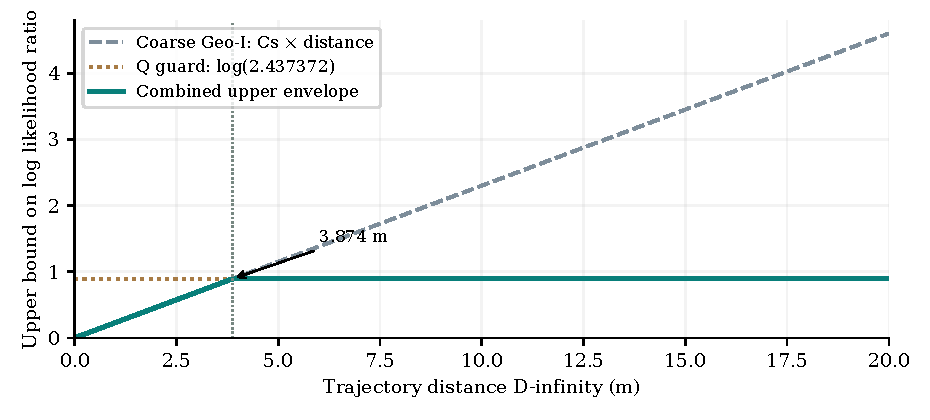
\includegraphics[width=.86\linewidth]{figure_bound_profile.pdf}
\caption{Illustrative upper envelopes for the frozen parameters, not an
empirical privacy curve. The minimum uses both sets of assumptions.
The spatial term is coarse; the dimensionless Q guard dominates beyond
approximately 3.874 m.}\label{fig:bound-profile}
\end{figure}

\begin{corollary}[Arbitrary-estimator localization]\label{cor:hit}
At the same context $C$, suppose the Q ratio bound $R$ holds uniformly over the
support of a valid trajectory prior. Define
$\pi_{\max,t}(r)=\sup_y\Pr(\|X_t-y\|_2\le r\mid C)$. Every measurable estimator
$\widehat x_t(O)$ satisfies
\begin{equation}
\Pr(\|X_t-\widehat x_t(O)\|_2\le r\mid C)
\le \frac{R\pi_{\max,t}(r)}{1+(R-1)\pi_{\max,t}(r)}. \label{eq:hit}
\end{equation}
\end{corollary}
\begin{proof}
For a realized output $o$, fix the private-input event inside the radius-$r$
ball centered at $\widehat x_t(o)$. Mixture likelihood ratios give the posterior-odds
ceiling $f_R(\pi)=R\pi/[1+(R-1)\pi]$ for that event. Its prior is at most
$\pi_{\max,t}(r)$, and $f_R$ is increasing. Integrating over outputs proves the
claim. Weighted time averages follow by linearity without independent errors.
Finite/countable outputs, or an appropriate common-density version, are understood.
\end{proof}
Choosing $r=100$ m links the theorem to Hit100, but does not infer its empirical
value from the theorem. A strong spatial prior can make the bound uninformative.
In a balanced binary illustration, the one-session ceiling corresponds to posterior
at most approximately 70.91\%, not to an asserted average attack accuracy.

\begin{corollary}[Conditional joint channels]\label{cor:joint}
If each of $m$ channels has a conditional ratio bound $R_\ell$ at every feasible
common joint prefix, their joint transcript has ratio at most $\prod_\ell R_\ell$.
Private inputs may be correlated.
\end{corollary}
Chain rule proves the statement; marginal per-channel guarantees alone are not its
assumption. Two valid $\Gamma_Q=1$ channels give a balanced-prior posterior ceiling
below 85.5925\%, rather than the one-session 70.91\%. A Raw partner lacks the required
finite guard. Likewise, $\Gamma_Q=0$ yields $p=w$ at every prefix, so its wire law is
independent of the private trajectory at fixed context under the public-channel
assumptions. Positive adaptation is a permitted design choice, not a privacy necessity.

\subsection{Utility properties and their scope}\label{sec:utility}
At the same local state, let $r_a\in[0,1]$ denote actual conditional utility of action
$a$. Centering gives, for any vector $f$,
$\E_pf-\E_wf=\alpha\Cov_w(z,f)$. In particular,
\begin{align}
\E_pz-\E_wz&=\alpha\Var_w(z)\ge0,\\
\E_pr-\E_wr&=\alpha\Cov_w(z,r). \label{eq:gain}
\end{align}
For a proxy $v$ satisfying $\max_a|r_a-v_a|\le\eta$,
\begin{equation}
\E_pr-\E_wr\ge\alpha\{\Cov_w(z,v)-\eta\E_w|z-\E_wz|\}. \label{eq:calibration}
\end{equation}
The uncertainty in $\eta$ cannot be set to zero because belief uses Bayes' rule.
The nonnegative score gain is not a nonnegative actual Recall gain.

Let $T_t$ be the full-catalogue reference top-$k$ after filtering and deterministic
tie-breaking, and $U_t$ the valid received metadata. Local top-$k$, used for evaluation
only, obeys
\begin{equation}
\operatorname{Recall@}k=\frac{|T_t\cap U_t|}{|T_t|},\qquad T_t\ne\varnothing. \label{eq:recall}
\end{equation}
Every received reference item precedes every non-reference item in the same order.
Thus it survives local top-$k$, proving (\ref{eq:recall}). Set inclusion of valid
caches cannot reduce Recall at the same GPS/request. It does not imply monotone
Recall while GPS or requests change, nor does ranking create missing metadata.

For a whole-session comparison, let $P_n$ be the adaptive history law and $W_n$ the
\emph{identical} public policy with $\Gamma_Q=0$, including the same provider and
external conditions. At each fixed prefix,
$\chi^2(p_j\Vert w_j)=\alpha_j^2\Var_{w_j}(z_j)\le\alpha_j^2/4$.
If the protected score remains latent at that prefix, $z_j$ here denotes its
conditional mean under the adaptive law; it is still bounded in $[0,1]$.
A conditional second-moment recursion then yields, for every $h\in[0,1]$,
\begin{align}
|\E_{P_n}h-\E_{W_n}h|
&\le\TV(P_n,W_n)\\
&\le\frac12\sqrt{\prod_{j\le n}(1+\alpha_j^2/4)-1}. \label{eq:tv}
\end{align}
For $\Gamma_Q=1$, a rational tail certificate gives a uniform ceiling below
0.0553. This bounds a possible difference from a matched base, not absolute
utility or superiority to another paper. The sign remains empirical.

Finally, at a fixed history, let $\rho$ be a declared public case law and $\lambda$
the actual case law. If $\E_\rho\widehat r\ge c$,
$\TV(\lambda,\rho)\le\tau$ and $\E_\lambda|r-\widehat r|\le\nu$, then
\begin{equation}
\E_\lambda r\ge\max\{0,c-\tau-\nu\}. \label{eq:floor}
\end{equation}
Conditional expectation and public time weights extend this to a session without
IID assumptions. The supplement gives exact nonvacuous finite examples and a
negative actual-gain counterexample. Real-provider calibration is not certified
by these illustrations.

Purpose-independent payloads supply a separate interface property: changing $\psi$
at fixed trajectory, context and randomness does not change the cover request.
This conditional noninterference does not remove intent correlated with location.
The complete practical guarantee still depends on state persistence, entropy,
numerical support and absence of additional side channels. Floating-point privacy
implementations require care~\cite{mironov}; our ideal analysis and integer Q
representation are not a complete deployment certificate.

\section{Experiments and analysis}\label{sec:evaluation}
\subsection{Workload, splits and service contract}
The controlled workload uses native SUMO mobility~\cite{sumo}, a versioned directed
road graph derived from public geographic inputs, and 418 POIs in six categories
with OpenStreetMap provenance~\cite{osm}. The graph contains 66,189 road states,
4,849 external edges and 21,179 internal edges. The compiled native network is
not asserted to reproduce every original Beijing lane or junction.

The source cohort has 48 route families. The experiment retains days 7 and 8
and a 600-second window with 31 service ticks at 20-second spacing. Families
are disjoint across 20 TRAIN, 8 SELECTION and 20 TEST groups. TRAIN/SELECTION
use one retained draw per native trip; TEST uses three, giving 120 trip-draws
per arm from 40 test trips. Repeated draws are not independent route families.
Eligibility uses declared road geometry and route-calibration rules rather
than defense protection scores. This cohort and map were inspected during
development; the study is not a fresh-city or untouched-geometry confirmation.

All arms use the same catalogue, $L=60$ per category/coordinate, local filters,
reference costs and tie-breaking. The four purposes minimize road distance,
minimize travel time, filter within 1,000 m and rank by distance, or minimize
detour to a private local destination. A reference contains up to five items.
The application answer itself is not truncated to five. Empty references remain
not applicable (N/A), with their denominators retained.

We distinguish current-packet, 60-second epoch and whole-session caches.
The principal utility result uses a static session cache. The provider's
complete reply signatures are public design resources and match the
experimental provider. This controlled condition is essential to interpreting
the high coverage and does not establish a need for repeated remote acquisition.

\subsection{Comparisons and attack protocol}
\begingroup\footnotesize
\begin{longtable}{@{}P{2.7cm}P{3.6cm}P{7.3cm}@{}}
\caption{Controls, adaptations and the frozen proposed method.}\label{tab:methods}\\
\toprule\textbf{Method} & \textbf{Public output contract} & \textbf{Configuration / fidelity} \\
\midrule\endfirsthead
\multicolumn{3}{l}{\textit{Continued from previous page}}\\
\toprule\textbf{Method} & \textbf{Public output contract} & \textbf{Configuration / fidelity} \\
\midrule\endhead
\midrule\multicolumn{3}{r}{\textit{Continued on next page}}\\\endfoot
\bottomrule\endlastfoot
Raw GPS & One real coordinate & Unprotected control \\
REM-Z (K1) & One REM coordinate & $u=0.01\,\mathrm m^{-1}$; frozen references \\
TransProtect* & One replacement coordinate & Markov predictor; $K=10$, 8 TRAIN targets, $\alpha_{\rm TP}=10000$, $\varepsilon=0.005\,\mathrm m^{-1}$ \\
Semantic* & True point + 4 dummies & OSM/empirical predictor; candidate pool 128; replaces AMap/LSTM \\
Fake queries* & K5 sets + inserted fake events & Road/history predictor; up to 2 fake events, waits 5--15 s, 24 candidates, similarity 0.75 \\
\textbf{GeoI-BQ v1} & K5 committed frames & $\Gamma_Q=1$, $C_s=0.23\,\mathrm m^{-1}$; protected read interval $\ge60$ s \\
\end{longtable}
The methods have different guarantees, output cardinalities and costs. We do not equate their epsilon values.
\endgroup

Table~\ref{tab:methods} lists six implementations. The three starred methods
are audited adaptations with declared substitutions, not official author
reproductions or matched-privacy-budget executions. GeoI-BQ and direct REM-Z
replay their frozen coordinates and timestamps without favorable resampling.
Fake-query insertion retains all naturally emitted extra packets.

The attack bank includes geometry/history estimators, ExtraTrees with 64
trees~\cite{extratrees}, shadow kNN-1/kNN-5 and priors. Endpoint tasks add
ordered and geometry-linked sequences. Models fit TRAIN; robust selection on
SELECTION is separate for each method, task and loss, using mean plus standard
error for MAE and mean minus standard error for Hit. TEST never supplies
estimator features, true-member flags, internal $Z$, belief or evaluator indices.
Hit and MAE in the same cell may therefore come from different selected estimators.
For GeoI-BQ, the principal Hit100 selector chooses centroid in all five tasks;
MAE selects prior-based estimators. This is not evidence that a Bayes-optimal
attacker failed.

S1 observes one packet at a service tick. S2 observes all wire from 540 to
600 seconds and targets the mean of four final GPS ticks, a coordinate proxy
rather than semantic home/work inference. S3 uses the complete 0--600-second
wire to reconstruct the 31 target positions. S9 and S10 estimate the first
and last GPS from the full wire with known public boundaries. Comparisons use
the same time window, not the same number of packets; auxiliary fake events
remain visible and are charged.

For error $e_i=\|x_i-\widehat x_i\|_2$, the principal privacy metrics are
$\operatorname{Hit100}=N^{-1}\sum_i\mathbf1_{\{e_i\le100\}}$ and
$\operatorname{MAE}=N^{-1}\sum_i e_i$. Lower Hit and higher MAE favor protection
within the declared task. S3 Hit is pointwise reconstruction performance
aggregated over time, not a whole-route success probability. Utility uses
(\ref{eq:recall}) and equal-purpose macro averaging over defined references.
Values aggregate within trip, then family, then across test families.
We use 10,000 paired family bootstrap replicates for 95\% percentile
intervals~\cite{efron}. Intervals condition on the retained cohort and models;
they do not capture all dataset-generation, selection or domain-shift uncertainty.
Failures retain coverage and are not counted as successful privacy.

\subsection{Localization, utility and cost}
\begin{table}[htbp]\centering\footnotesize
\caption{Localization results: Hit100 (\%, lower) / MAE (m, higher). Same time windows.}\label{tab:privacy}
\begin{tabularx}{\linewidth}{@{}P{2.7cm}YYYYY@{}}\toprule
\textbf{Method} & \textbf{S1} & \textbf{S2} & \textbf{S3} & \textbf{S9} & \textbf{S10} \\
\midrule
Raw GPS & \shortstack[l]{100.000 /\\ 0.0} & \shortstack[l]{100.000 /\\ 0.0} & \shortstack[l]{100.000 /\\ 0.0} & \shortstack[l]{100.000 /\\ 0.0} & \shortstack[l]{100.000 /\\ 0.0} \\
REM-Z (K1) & \shortstack[l]{18.522 /\\ 338.5} & \shortstack[l]{37.500 /\\ 214.3} & \shortstack[l]{18.522 /\\ 338.5} & \shortstack[l]{5.833 /\\ 435.8} & \shortstack[l]{35.000 /\\ 246.8} \\
TransProtect* & \shortstack[l]{82.984 /\\ 54.4} & \shortstack[l]{94.167 /\\ 28.7} & \shortstack[l]{82.984 /\\ 54.4} & \shortstack[l]{96.667 /\\ 17.8} & \shortstack[l]{90.833 /\\ 33.6} \\
Semantic* & \shortstack[l]{82.258 /\\ 41.9} & \shortstack[l]{100.000 /\\ 8.2} & \shortstack[l]{82.258 /\\ 41.9} & \shortstack[l]{100.000 /\\ 5.3} & \shortstack[l]{100.000 /\\ 7.3} \\
Fake queries* & \shortstack[l]{53.387 /\\ 1213.0} & \shortstack[l]{92.500 /\\ 239.1} & \shortstack[l]{98.790 /\\ 13.3} & \shortstack[l]{99.167 /\\ 42.2} & \shortstack[l]{100.000 /\\ 6.4} \\
\textbf{GeoI-BQ v1} & \shortstack[l]{0.188 /\\ 2104.6} & \shortstack[l]{0.000 /\\ 2124.2} & \shortstack[l]{0.188 /\\ 2104.6} & \shortstack[l]{0.000 /\\ 1986.4} & \shortstack[l]{0.000 /\\ 2124.2} \\
\bottomrule\end{tabularx}
\par\smallskip\raggedright * Audited adaptations, not official author implementations. Each loss has its own selected attacker. Full CIs appear in the supplement.
\end{table}

Table~\ref{tab:privacy} reports the five principal tasks. Raw recovers every
coordinate target with Hit100 100\%, establishing that the evaluation exposes
directly observed coordinates. GeoI-BQ has Hit100 0--0.188\% and MAE
1.99--2.12 km in the selected bank. Direct REM-Z remains more identifiable,
with Hit100 5.833--37.500\%.

The contrast with Fake-query insertion is instructive. Its S1 MAE is
1,213 m while Hit100 is still 53.387\%; with the whole S3 window,
Hit100 rises to 98.790\% and MAE falls to 13.3 m.
Additional fake events do not prevent a history-aware observer from exploiting
the known service clock in this adaptation. GeoI-BQ instead releases Q-only
actions from a broadly supported public library with bounded private tilting.
These are observations about the retained implementations, not universal
rankings of the original papers.

Zero-hit observations and degenerate bootstrap intervals do not imply zero
population risk. A large MAE also reflects the prior ambiguity and public
library geometry in this cohort; it is not a guaranteed noise displacement.
Full confidence intervals and selected estimators are supplied in the supplement.

\begin{table*}[t]\centering\footnotesize
\caption{Session-cache Recall@5 (\%, higher). The application returns a full sorted list.}\label{tab:utility}
\begin{tabularx}{\linewidth}{@{}P{2.7cm}YYYYY@{}}\toprule
\textbf{Method} & \textbf{Macro} & \textbf{Nearest} & \textbf{Fastest} & \textbf{Radius} & \textbf{Detour} \\
\midrule
Raw GPS & 99.999 & 100.000 & 100.000 & 100.000 & 99.995 \\
REM-Z (K1) & 99.700 & 99.753 & 99.753 & 99.625 & 99.668 \\
TransProtect* & 99.996 & 100.000 & 100.000 & 100.000 & 99.986 \\
Semantic* & 99.999 & 100.000 & 100.000 & 100.000 & 99.997 \\
Fake queries* & 99.999 & 100.000 & 100.000 & 100.000 & 99.997 \\
\textbf{GeoI-BQ v1} & 99.595 & 99.638 & 99.641 & 99.388 & 99.712 \\
\bottomrule\end{tabularx}
\end{table*}

GeoI-BQ achieves macro Recall 99.595\%, CI95\% [99.224, 99.903]\%.
It is approximately 0.4 percentage points below the three adaptations.
Against TransProtect*, the paired difference is $-0.401$ percentage points,
CI95\% [$-0.773$, $-0.093$]. Radius is the most sensitive purpose.
We retain the adverse sign and do not claim utility superiority.

\begingroup\footnotesize
\begin{longtable}{@{}P{2.7cm}P{2.2cm}P{2.2cm}P{2.2cm}P{2.2cm}@{}}
\caption{Mean wire cost per 600-second session; KB denotes 1,000 bytes.}\label{tab:cost}\\
\toprule\textbf{Method} & \textbf{Packets} & \textbf{Coordinates} & \textbf{Request KB} & \textbf{Reply KB} \\
\midrule\endfirsthead
\multicolumn{5}{l}{\textit{Continued from previous page}}\\
\toprule\textbf{Method} & \textbf{Packets} & \textbf{Coordinates} & \textbf{Request KB} & \textbf{Reply KB} \\
\midrule\endhead
\midrule\multicolumn{5}{r}{\textit{Continued on next page}}\\\endfoot
\bottomrule\endlastfoot
Raw GPS & 31.00 & 31.00 & 5.846 & 16.843 \\
REM-Z (K1) & 31.00 & 31.00 & 6.352 & 16.921 \\
TransProtect* & 31.00 & 31.00 & 6.351 & 16.847 \\
Semantic* & 31.00 & 155.00 & 31.754 & 84.770 \\
Fake queries* & 38.04 & 190.21 & 39.418 & 104.033 \\
\textbf{GeoI-BQ v1} & 31.00 & 155.00 & 31.756 & 82.557 \\
\end{longtable}
Request/reply serialization is the replay contract; reply bytes encode POI indices, not full production records, TLS or network energy.
\endgroup

Each 600-second session uses 155 coordinate queries for GeoI-BQ, compared with
31 for singleton controls and TransProtect*, 155 for Semantic*, and about
190.21 for Fake-query insertion*. The last arm emits approximately 38.04
packets rather than 31. Byte measurements serialize request/reply-index JSON:
they exclude full POI metadata, HTTP/TLS, radio latency and energy.
Generation timing for replayed GeoI-BQ and REM-Z is unavailable in this trial.
Shared service replay timings are not comparable device latency measurements.

\begin{figure}[htbp]\centering
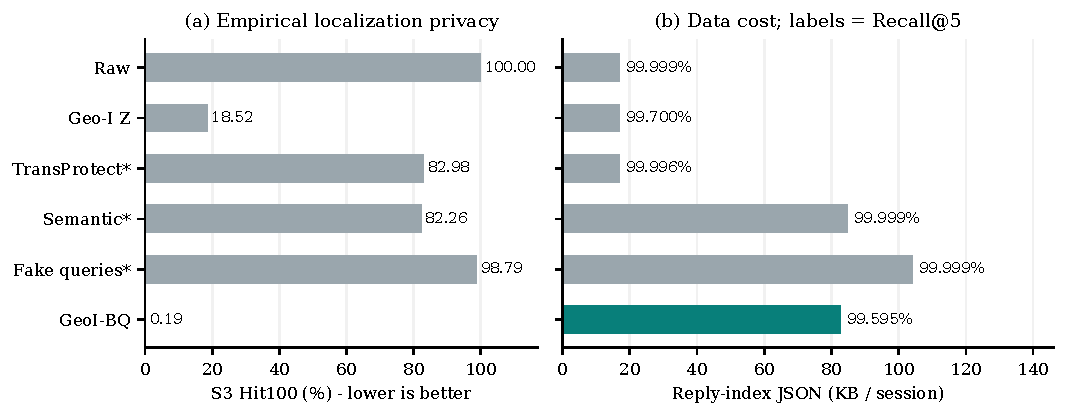
\includegraphics[width=\linewidth]{figure_tradeoff.pdf}
\caption{Controlled privacy--utility--cost comparison. Left: S3 Hit100
(lower favors protection). Right: reply-index JSON cost, with session
Recall labels. Starred methods are adaptations; neither equal cost nor
equal formal privacy is assumed.}\label{fig:tradeoff}
\end{figure}

\subsection{Original metrics and supplementary inference tasks}
The original-metric comparison is partial. The S3 point-error measure has
the expected-distance form of EIE, but does not reproduce TransProtect's
VehiTrack attack. For singleton outputs, its Equation-13 travel-cost
distortion is evaluated with eight TRAIN-selected targets/prior and directed
road distances: TransProtect* yields 47.44 m and REM-Z 688.65 m.
This is a local-target proxy, not experimental parity with the original
Rome/San Francisco study. GeoI-BQ has no unique released singleton to use
in that expression; selecting a secret-nearest Q would be invalid.
Real-member ASR, dummy-effectiveness DER and source-compatible path counts
remain unavailable or inapplicable for explicitly different reasons.
The supplement separates original metrics, task-aligned proxies, missing
reproduction inputs and incompatible contracts.

\begin{table*}[t]\centering\footnotesize
\caption{Extended diagnostics (\%); lower inference is preferable, subject to task validity.}\label{tab:scenario-summary}
\begin{tabularx}{\linewidth}{@{}P{2.7cm}YYY@{}}\toprule
\textbf{Method} & \textbf{S4 balanced acc.} & \textbf{S6 post-turn acc.} & \textbf{S8 protected-partner Hit100} \\
\midrule
Raw GPS & 100.00 & 100.00 & 100.00 \\
REM-Z (K1) & 91.67 & 50.00 & 6.67 \\
TransProtect* & 99.17 & 95.00 & 64.17 \\
Semantic* & 100.00 & 95.00 & 75.00 \\
Fake queries* & 93.33 & 99.17 & 68.33 \\
\textbf{GeoI-BQ v1} & 47.50 & 50.83 & 0.00 \\
\bottomrule\end{tabularx}
\par\smallskip\raggedright S4 is route-family association, not verified person/vehicle identity. S6 has two candidates (50\% chance). S8 is the post-V1 fusion diagnostic on the inspected cohort.
\end{table*}

Table~\ref{tab:scenario-summary} summarizes additional tasks; full six-arm
results are in the supplement. S4 is balanced route-family association,
not physical person/vehicle re-identification. GeoI-BQ's balanced accuracy
is 47.50\%, CI95\% [40.00, 54.17]\%. S5's Raw accuracy is 50\%:
the cadence misses informative turn observations, so its chance-level defense
score cannot establish a protection contribution. S6's post-turn two-destination
task is more informative: Raw achieves 100\%, adaptations 95--99.17\%,
and GeoI-BQ 50.83\%, CI95\% [44.17, 57.50]\%. REM-Z also achieves 50\%,
so this does not isolate a benefit from the Q layer.

S7 changes four purposes and six categories at fixed trajectory/context.
All 1,056 streams have equal wire across 25,344 counterfactuals. The joint
conditional Bayes vulnerability is $1/24$ under the balanced test prior.
All arms share this cover wrapper; it is not a unique advantage over the
papers' original interfaces or a natural-intent attack result.

S8 aligns two correlated synthetic native prefixes, grants channel association,
and evaluates target-only, protected-partner, Raw-partner and unrelated-partner
views. A stronger post-readout fusion bank increases Semantic* Hit100 from
45\% to 75\% and Fake-query* from 16.67\% to 68.33\%; GeoI-BQ has no hits
in the retained protected-partner sample. With a perfectly aligned Raw partner,
an available direct estimator attains 100\% in every arm. This is a diagnostic
of strong side information, not native simultaneous co-travel or independent
confirmation. The weaker bank and initial verifier-gate failure remain preserved.

\subsection{Attribution and limits of the application claim}
High Recall is explained partly by the small static catalogue and response
depth. Five coordinates times six categories times $L60$ permit up to
1,800 reply entries before deduplication against only 418 POIs.
A read-only audit of all 120 retained TEST draws finds 380.2 unique POIs
in the first GeoI-BQ packet on average (range 379--383), and 415.875 in the
final session cache (403--418): approximately 91\% and 99.49\% of the catalogue.
Current-packet Recall is 96.780\%, epoch-cache Recall 97.123\%, and
session-cache Recall 99.595\%. This is evidence of effective acquisition
and cache use under the contract, but weakly discriminates private planning
from broad public cover.

The matched public base $\Gamma_Q=0$ achieves 99.711\% Recall, exceeding
the primary policy by about 0.116 percentage points; the original paired
interval for primary minus base is [$-0.253$, $-0.006$] percentage points.
This supports the unfavorable direction in the observed cohort, not universal
dominance. It also agrees with (\ref{eq:gain}): score gain alone is insufficient.
We retain the policy family and its accounting without declaring private
adaptation necessary or optimal.

The data-access audit is stronger than a hypothetical bulk-API objection:
the prototype itself loads complete reference data sufficient for the four
static objectives. Therefore online necessity is not established against a
client allowed to use that information directly. A deployment must distinguish
offline design resources from genuinely unavailable current metadata and
measure acquisition/setup/refresh costs for an equally informed control.
The current offline-information result is analytical, not a measured seventh
arm with zero total system cost.

Duration is another untested regime. At most 11 protected reads fit the
0--600-second clock; worst-case spend is $1+2(11-1)=21<23$ units.
All retained ledgers end at 13--21 units, with no cap exhaustion.
The duration-independent privacy accounting consequently has not been
paired with an empirical utility test after new protected GPS is disallowed.

Finally, the theory is conditional on common support, fixed/public boundary
rules, provider laws and valid state handling. Integer Q sampling does not
certify floating-point REM, practical entropy or full upstream restoration.
Physical identity, correlated intent, user feedback and linked sessions
require their own conditions. These limitations constrain the interpretation
of the results; they are not erased by low empirical Hit100.

\section{Conclusion}\label{sec:conclusion}
GeoI-BQ separates protected spatial information from public query actions and
accounts for both across a stateful LBS session. Under explicit assumptions,
REM and a private reuse test provide a spatial history bound, while a
common-support segment kernel supplies an independent summable transcript
guard. Their combination yields a conditional end-to-end guarantee.
Prior concentration connects the guard to arbitrary-estimator localization;
conditional composition extends the reasoning to joint channels without
assuming independent private movement.

Utility has a different status: exact local-ranking/cache properties and
bounded perturbation relative to a matched public base are proved, while
absolute service floors depend on quantified proxy and distribution errors.
The controlled synthetic comparison exhibits low localization Hit100 and
99.595\% session Recall at 155 coordinate queries per 600 seconds, with a
small utility loss relative to three audited paper adaptations.
It also exposes limits: a stronger public-base control, near-complete
catalogue acquisition, complete prototype reference access and an
unexercised post-cap regime.

The supported contribution is thus a specified and auditable bounded
publication mechanism, its connected conditional analysis, and a reproducible
evaluation with explicit unfavorable evidence. Deployment certification,
faithful original-paper reproduction, independently registered mobility
cohorts and genuinely unknown or changing provider records remain separate
requirements for stronger claims of practical advantage.

\section*{Data and code availability}
Synthetic mobility, geographic snapshots, code and frozen artifact hashes are indexed
by the accompanying manifest. Original geographic licenses apply.
A persistent publication archive remains to be registered.
\section*{Declaration of generative AI assistance}
OpenAI ChatGPT/Codex assisted drafting, software preparation and consistency checks.
The authors remain responsible for final verification, editing and approval.
\begin{thebibliography}{99}
\bibitem{mobilityunique} Y.-A. de Montjoye, C. A. Hidalgo, M. Verleysen and V. D. Blondel. Unique in the Crowd: The privacy bounds of human mobility. Scientific Reports 3, 1376, 2013. \href{https://doi.org/10.1038/srep01376}{doi:10.1038/srep01376}.
\bibitem{geoi} M. E. Andrés, N. E. Bordenabe, K. Chatzikokolakis and C. Palamidessi. Geo-Indistinguishability: Differential Privacy for Location-Based Systems. ACM CCS 2013, pp.901--914. \href{https://arxiv.org/abs/1212.1984}{Author version}.
\bibitem{predictive} K. Chatzikokolakis, C. Palamidessi and M. Stronati. A Predictive Differentially-Private Mechanism for Mobility Traces. Privacy Enhancing Technologies 2014. \href{https://petsymposium.org/2014/papers/Chatzikokolakis.pdf}{Author version}.
\bibitem{ev} U. I. Atmaca, S. Biswas, C. Maple and C. Palamidessi. A privacy-preserving querying mechanism with high utility for electric vehicles. IEEE Open Journal of Vehicular Technology 5:262--277. 2024. \href{https://wrap.warwick.ac.uk/id/eprint/183198/}{DOI: 10.1109/OJVT.2024.3360302}.
\bibitem{transprotect} S. Yadav, C. Yu, X. Xie, Y. Huang and C. Qiu. Protecting Vehicle Location Privacy with Contextually-Driven Synthetic Location Generation. ACM SIGSPATIAL 2024. \href{https://arxiv.org/abs/2409.09495}{DOI: 10.1145/3678717.3691211}.
\bibitem{semantic} H. Liu, H. Peng and N. Zhou. A dummy-based location privacy protection scheme with semantic correlation of moving paths. Journal of King Saud University Computer and Information Sciences 38:478. 2026. \href{https://link.springer.com/article/10.1007/s44443-026-00899-w}{DOI: 10.1007/s44443-026-00899-w}.
\bibitem{fake} H. Liu, S. Hu and N. Zhou. Location privacy protection in continuous LBSs: enhancing anonymity via fake queries. Journal of King Saud University Computer and Information Sciences 38:53. 2026. \href{https://link.springer.com/article/10.1007/s44443-025-00438-z}{DOI: 10.1007/s44443-025-00438-z}.
\bibitem{sok} E. Buchholz, A. Abuadbba, S. Wang, S. Nepal and S. S. Kanhere. SoK: Can Trajectory Generation Combine Privacy and Utility?. Proceedings on Privacy Enhancing Technologies 2024(3):75--93. \href{https://petsymposium.org/popets/2024/popets-2024-0068.pdf}{DOI: 10.56553/popets-2024-0068}.
\bibitem{dworkroth} C. Dwork and A. Roth. The Algorithmic Foundations of Differential Privacy. Foundations and Trends in Theoretical Computer Science 9(3--4), 211--407, 2014. \href{https://doi.org/10.1561/0400000042}{doi:10.1561/0400000042}. Author version: \url{https://www.cis.upenn.edu/~aaroth/Papers/privacybook.pdf}.
\bibitem{ptppm} M. Min et al.. Road Network-Aware Personalized Trajectory Protection with Differential Privacy under Spatiotemporal Correlations. arXiv:2511.21020, preprint. 2025. \href{https://arxiv.org/abs/2511.21020}{DOI: 10.48550/arXiv.2511.21020}.
\bibitem{iwpe26} L. Santos, M. Cunha and J. Vilela. Location Privacy Protection through Road Network Adaptability and User Mobility Prediction. IWPE 2026 program abstract, 6 July 2026. \url{https://www.iwpe.info/program.html}. Program abstract only; no full-paper reproduction claimed.
\bibitem{cpcrok} J. Wang, H. Li, Y. Sun, C. Phillips, A. Mylonas and D. Gritzalis. CPCROK: A Communication-Efficient and Privacy-Preserving Scheme for Low-Density Vehicular Ad Hoc Networks. Future Internet 17(4):165. 2025. \href{https://uhra.herts.ac.uk/id/eprint/25705/}{DOI: 10.3390/fi17040165}.
\bibitem{dpfetc} B. Yue, S. Li, A. Liu and X. Li. DP-FETC: a differentially private trajectory publishing method based on feature extraction and trajectory correlation. Electronic Research Archive 33(11):6631--6651. 2025. \href{https://www.aimspress.com/article/doi/10.3934/era.2025293}{DOI: 10.3934/era.2025293}.
\bibitem{mironov} I. Mironov. On Significance of the Least Significant Bits for Differential Privacy. ACM CCS, 650--661, 2012. \href{https://doi.org/10.1145/2382196.2382264}{doi:10.1145/2382196.2382264}. Author version: \url{https://www.microsoft.com/en-us/research/publication/on-significance-of-the-least-significant-bits-for-differential-privacy/}.
\bibitem{sumo} P. Alvarez Lopez, M. Behrisch, L. Bieker-Walz, J. Erdmann, Y.-P. Flötteröd, R. Hilbrich, L. Lücken, J. Rummel, P. Wagner and E. Wießner. Microscopic Traffic Simulation using SUMO. IEEE ITSC, 2575--2582, 2018. \href{https://doi.org/10.1109/ITSC.2018.8569938}{doi:10.1109/ITSC.2018.8569938}. Citation guidance: \url{https://sumo.dlr.de/docs/FAQ.html}.
\bibitem{osm} OpenStreetMap contributors. OpenStreetMap: Copyright and License. \url{https://www.openstreetmap.org/copyright/}. Accessed 9 November 2026; geographic snapshots are versioned in the research repository.
\bibitem{efron} B. Efron. Bootstrap Methods: Another Look at the Jackknife. The Annals of Statistics 7(1), 1--26, 1979. \href{https://doi.org/10.1214/aos/1176344552}{doi:10.1214/aos/1176344552}.
\bibitem{extratrees} P. Geurts, D. Ernst and L. Wehenkel. Extremely randomized trees. Machine Learning 63, 3--42, 2006. \href{https://doi.org/10.1007/s10994-006-6226-1}{doi:10.1007/s10994-006-6226-1}.

\end{thebibliography}
\end{document}
